\title{Лекция 16\\Методика коллективной разработки баз знаний}
\author[]{Шункевич Д.В.}
\institute[]{Белорусский государственный университет информатики и радиоэлектроники}

\begin{frame}
	\titlepage
\end{frame}

\begin{frame}{\\Содержание лекции}
	\topline
	\justifying
	Понятие разработчика базы знаний, виды разработчиков. Структуризация базы знаний с точки зрения разработчиков. Основные принципы взаимодействия разработчиков баз знаний. Верификация базы знаний, поиск неполноты.
\end{frame}


\begin{frame}{\\Общая идея разработки баз знаний}
	\topline
	\justifying
	\vspace{10mm}
	\begin{SCn}
		\begin{figure}[H]
			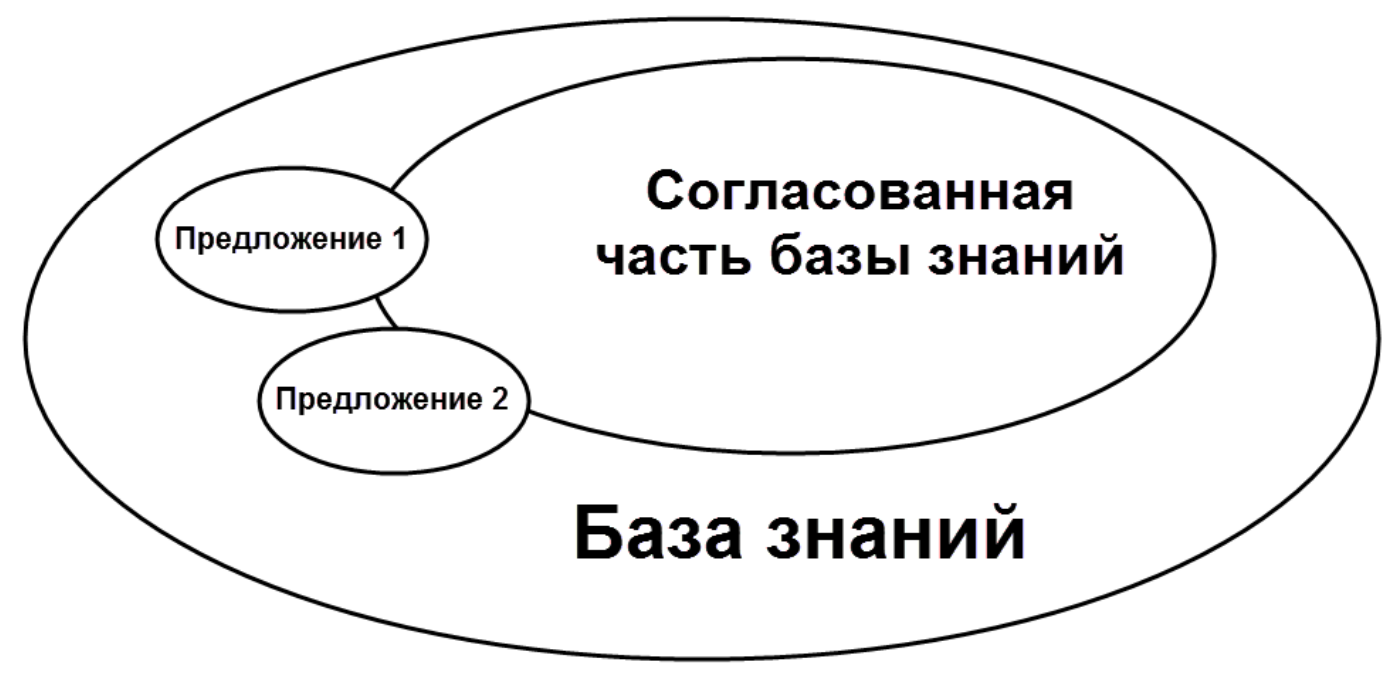
\includegraphics[scale=0.5]{./figures/sd_kb_develop_methods/kb_develop_idea.png}
		\end{figure}
	\end{SCn}
\end{frame}

\begin{frame}{\\Понятие незарегистрированного пользователя}
	\topline
	\justifying
	\begin{SCn}
		\scnheader{незарегистрированный пользователь*}
		\scnidtf{бинарное отношение, связывающее ostis-систему и sc-элемент, обозначающий персону, не прошедшую процедуру регистрации в системе}
		\vspace{5mm}
		
		\textbf{Права незарегистрированного пользователя:}
		\begin{textitemize}
			\item{доступ на чтение предметной части базы знаний ostis-системы}
			\item{работа	с ostis-системой в режиме эксплуатации}
		\end{textitemize}
	\end{SCn}
\end{frame}

\begin{frame}{\\Понятие зарегистрированного пользователя}
	\topline
	\justifying
	\begin{SCn}
		\scnheader{зарегистрированный пользователь*}
		\scnidtf{бинарное отношение, связывающее ostis-систему и sc-элемент, обозначающий персону, прошедшую процедуру регистрации в системе}
		\vspace{10mm}
	\end{SCn}
	\textbf{Права зарегистрированного пользователя:}
	\begin{textitemize}
		\item{доступ на чтение всей базы знаний}
		\item{внесение предложений ко всей базе знаний}
		\item{работа в режиме эксплуатации/разработчика}
	\end{textitemize}
\end{frame}

\begin{frame}{\\Понятие разработчика базы знаний}
	\topline
	\justifying
	\vspace{8mm}
	\begin{SCn}
		\scnheader{разработчик*}
		\scnsuperset{зарегистрированный пользователь*}
		\scnidtf{бинарное ориентированное отношение, связывающее какой-либо проект по разработке раздела базы знаний ostis-системы (в пределе -- всей базы	знаний) и sc-элемент, обозначающий персону, которая может быть разработчиком данного раздела базы знаний, т. е. выполнять проектные задачи в рамках данного раздела}
	\end{SCn}
	\bigskip
	\textbf{Права разработчика:}
	\begin{textitemize}
		\item{доступ на чтение всей базы знаний}
		\item{оставление комментариев к предложениям по редактированию базы знаний}
		\item{внесение предложений ко всей базе знаний}
		\item{работа в режиме эксплуатации/разработчика}
	\end{textitemize}
\end{frame}

\begin{frame}{\\Виды разработчиков. Роль администратор}
	\topline
	\justifying
	\begin{SCn}
	\vspace{5mm}
		\scnheader{разработчик*}
		\begin{scnrelfromset}{разбиение}
			\scnitem{администратор*}
			\scnitem{менеджер*}
			\scnitem{эксперт*}
		\end{scnrelfromset}
	\scnheader{администратор*}
	\scnrelfrom{включение}{бинарное ориентированное отношение}
	\scnrelfrom{первый домен}{проект по разработке раздела базы знаний ostis-системы}
	\scnrelfrom{второй домен}{sc-элемент, обозначающий персону, которая является администратором данного раздела базы знаний}
	\end{SCn}
\end{frame}

\begin{frame}{\\Задачи администратора}
	\topline
	\justifying
	\begin{SCn}
		\textbf{Задачами администратора являются:}
		\begin{textitemize}
			\item контроль целостности и непротиворечивости всей базы знаний;
			\item определение уровней доступа других пользователей;
			\item принятие решения относительно принятия или отклонения предложений в различные части базы знаний, в том числе при необходимости отправка их на экспертизу;
			\item самостоятельное внесение изменений в различные части базы знаний	путем использования соответствующих команд редактирования (при этом изменения автоматически оформляются как предложения и заносятся в раздел
			истории развития ostis-системы)	
		\end{textitemize}
	\end{SCn}
\end{frame}

\begin{frame}{\\Иерархия администраторов базы знаний}
	\topline
	\justifying
	\begin{SCn}
		При необходимости разработки объемной базы знаний может вводится иерархия разработчиков, соответствующая иерархии разделов разрабатываемой базы знаний.\\ 
	    В этом случае утверждение какого-либо предложения администратором раздела нижнего уровня не приводит к интеграции предложения в соответствующий раздел, а требует рассмотрения администраторами более	высокого уровня. \\ 
	    Окончательное решение принимается администратором всей базы знаний.
	\end{SCn}
\end{frame}

\begin{frame}{\\}
	\topline
	\justifying
	\vspace{10mm}
	\begin{SCn}
		\begin{figure}[H]
			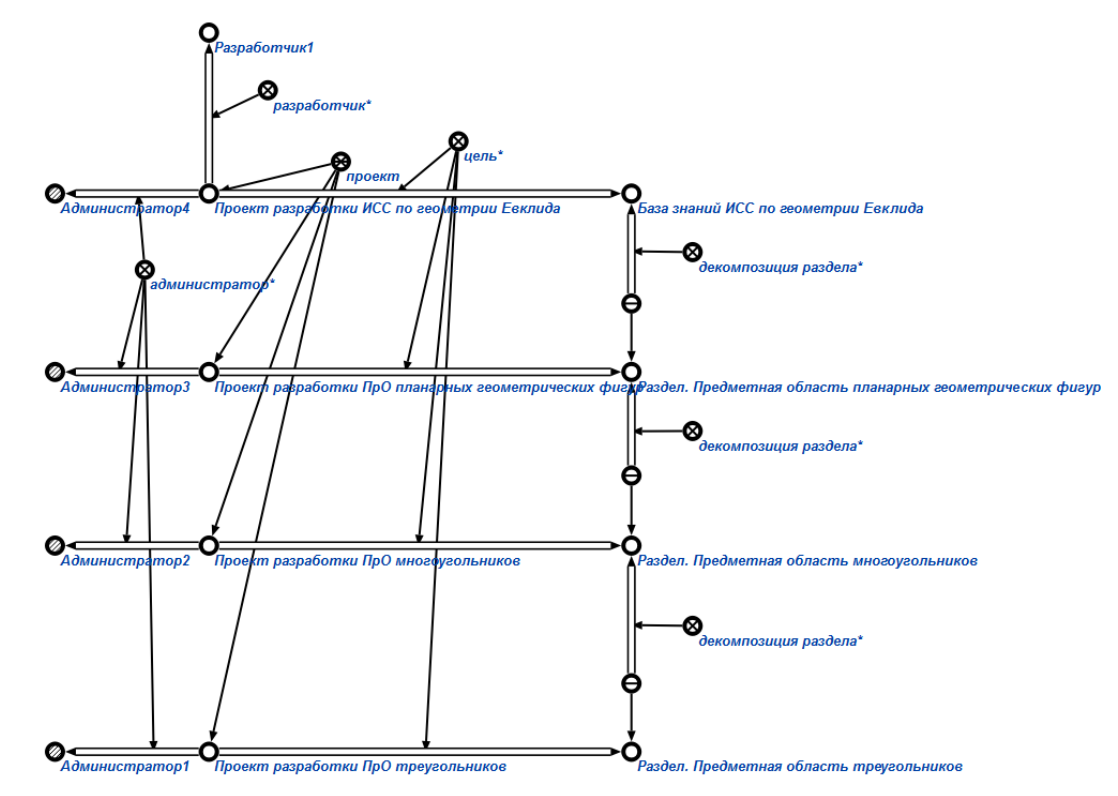
\includegraphics[scale=0.27]{./figures/sd_kb_develop_methods/hierarchy.png}
		\end{figure}
	\end{SCn}
\end{frame}

\begin{frame}{\\Роль менеджер}
	\topline
	\justifying
	\begin{SCn}
		\scnheader{менеджер*}
		\scnidtf{бинарное отношение, связывающее какой-либо проект по разработке раздела базы знаний ostis-системы (в общем случае -- всей базы знаний) и sc-элемент, обозначающий персону, которая является менеджером данного раздела базы знаний}
	\end{SCn}
	\textbf{Задачи менеджера:}
	\begin{textitemize}
		\item планирование объемов работ по разработке базы знаний;
		\item установка приоритетов и сроков выполнения задач;
		\item детализация проектных задач на подзадачи, формулирование проектных задач, назначение исполнителей проектных задач;
		\item контроль сроков выполнения проектных задач
	\end{textitemize}
\end{frame}

\begin{frame}{\\Роль эксперт}
	\topline
	\justifying
	\begin{SCn}
		\scnheader{эксперт*}
		\scnidtf{бинарное отношение, связывающее какой-либо проект
		по разработке раздела базы знаний ostis-системы и sc-элемент, обозначающий персону, которая является экспертом данного раздела базы знаний}
	\end{SCn}
	\textbf{Задачами эксперта являются:}
	\begin{textitemize}
		\item верификация результатов выполнения проектных задач;
		\item эксперт может оставлять комментарии к любому фрагменту базы знаний относительно его корректности. Кроме того, любой участник процесса разработки имеет возможность оставить естественно-языковой комментарий к любому фрагменту или элементу базы знаний, таким образом, может осуществляться обсуждение каких-либо вопросов, связанных с указанным фрагментом или элементом базы знаний. Такого рода комментарии попадают в раздел базы знаний \textit{текущие процессы развития ИС}.
	\end{textitemize}
\end{frame}

\begin{frame}{\\}
	\topline
	\justifying
	
	\begin{SCn}
		\begin{figure}[H]
			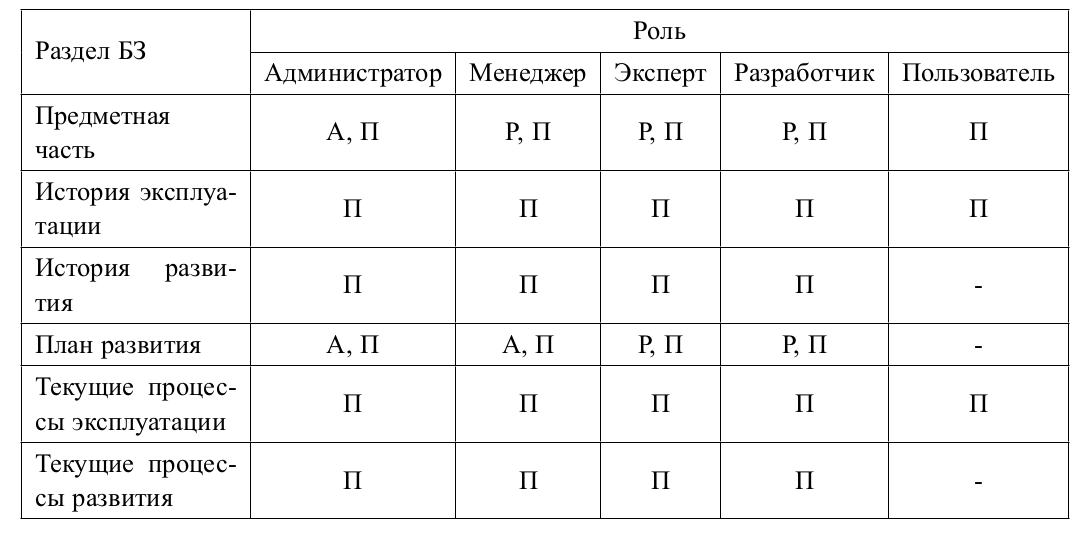
\includegraphics[scale=0.3]{./figures/sd_kb_develop_methods/table.png}
		\end{figure}
	\end{SCn}
\end{frame}

\begin{frame}{\\}
	\topline
	\justifying
	
	\begin{SCn}
		В ячейках таблицы отражено наличие	у соответствующих групп пользователей прав доступа на редактирование посредством формирования предложений (буква Р), просмотр (буква П) и редактирование с автоматическим формированием и принятием предложения по редактированию базы знаний (буква А).
	\end{SCn}
\end{frame}

\begin{frame}{Структуризация базы знаний с точки\\ зрения разработчиков.}
\topline
\justifying
\vspace{10mm}
\begin{SCn}
	\begin{figure}[H]
		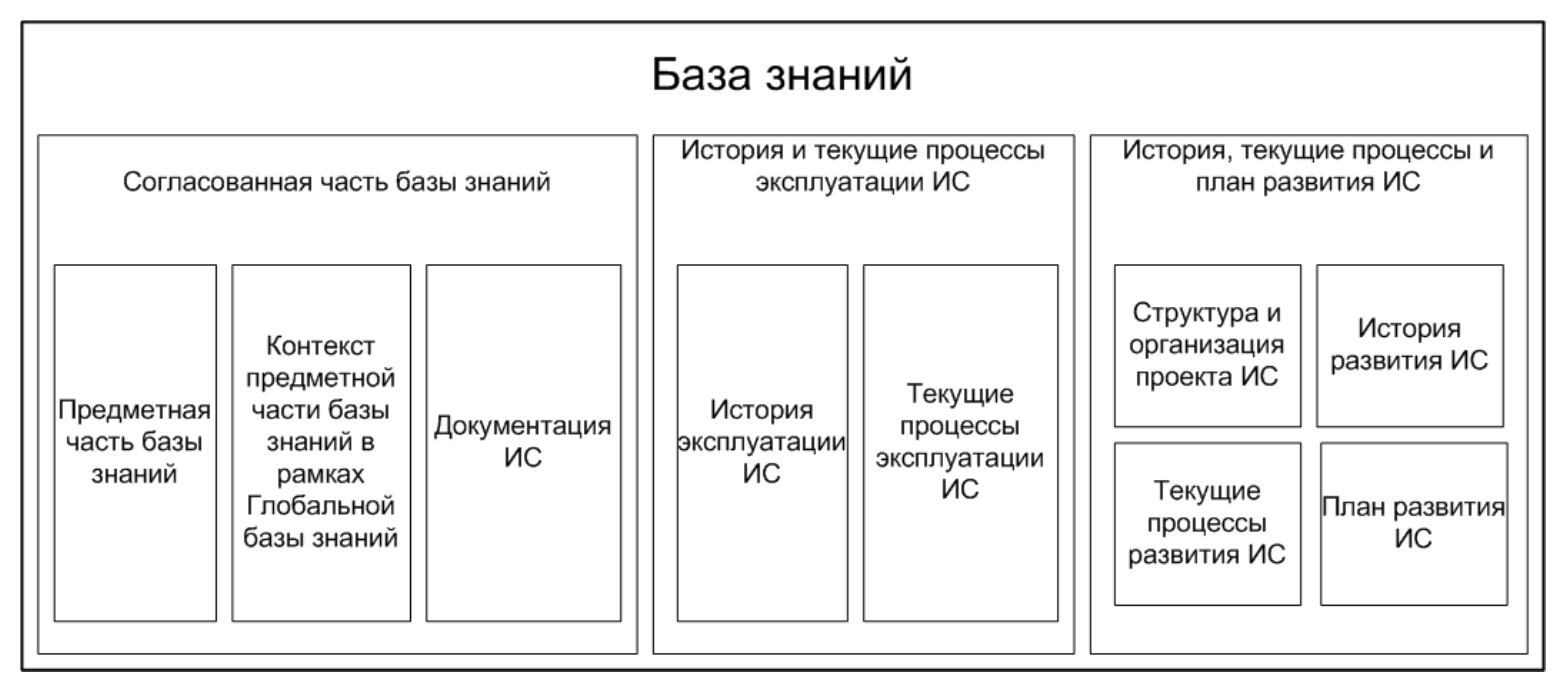
\includegraphics[scale=0.45]{./figures/sd_kb_develop_methods/kb_struct_develop.png}
	\end{figure}
\end{SCn}
\end{frame}


\begin{frame}{Структуризация базы знаний с точки\\ зрения разработчиков.}
	\topline
	\justifying
	\begin{SCn}
		\scnheader{база знаний}
		\begin{scnrelfromset}{разбиение}
			\scnitem{согласованная часть базы знаний}
			\scnitem{история и текущие процессы эксплуатации ИС}
			\scnitem{история, текущие процессы и план развития ИС}
		\end{scnrelfromset}
		\scntext{примечание}{Чтобы обеспечить эволюцию системы необходимо выделить специальные разделы базы знаний. Эти разделы содержат информацию о будущих планах развития системы, текущих и предыдущих процессах её разработки.}
	\end{SCn}
\end{frame}

\begin{frame}{\\Согласованная часть базы знаний}
	\topline
	\justifying
	\begin{SCn}
		\scnheader{согласованная часть базы знаний}
		\scnidtf{часть базы знаний, которая согласована между всеми участниками разработки в текущий момент времени}
		\scnidtf{часть базы знаний, доступная конечным пользователям системы в режиме эксплуатации системы}
		\scntext{примечание}{Выделение согласованной части базы знаний необходимо для того, чтобы иметь возможность скрыть от конечного пользователя системную информацию, не связанную непосредственно с эксплуатацией интеллектуальной системы.}
	\end{SCn}
\end{frame}

\begin{frame}{\\}
	\topline
	\justifying
	\vspace{5mm}
	\begin{SCn}
		\scnheader{согласованная часть базы знаний}
		\begin{scnrelfromset}{разбиение}
			\scnitem{предметная часть базы знаний}
			\scnitem{контекст предметной части БЗ в рамках Глобальной БЗ}
			\scnitem{документация ИС}
		\end{scnrelfromset}
	
		\scnheader{Глобальная база знаний}
		\scnidtf{глобальное абстрактное семантическое пространство всех знаний, накопленных человечеством к текущему моменту времени}
		
		\scnheader{предметная часть базы знаний}
		\scnidtf{часть базы знаний, которая содержит всю информацию о предметной области (или нескольких взаимосвязанных предметных областях в рамках БЗ), для работы с которой предназначена разрабатываемая система}
	\end{SCn}
\end{frame}

\begin{frame}{\\}
	\topline
	\justifying
	\begin{SCn}		
		\scnheader{контекст предметной части базы знаний в рамках Глобальной базы знаний}
		\scnidtf{спецификация объектов, которые не исследуются непосредственно в предметной части базы знаний данной системы, но имеют к ней	отношение, т. е., упоминаются при описании каких-либо понятий, исследуемых в предметной части базы знаний}
		\scntext{пример}{Для системы по Геометрии Евклида таким контекстом является историческая справка о жизни Евклида, математики и т. д.}
		
		\scnheader{документация компьютерной системы}
		\scnidtf{документация самой ostis-системы, спецификация ее базы знаний, машины	обработки знаний и интерфейса, а также все необходимые руководства, обеспечивающие возможность обучения работе с системой}
	\end{SCn}
\end{frame}

\begin{frame}{История и текущие\\ процессы эксплуатации ИС}
	\topline
	\justifying
	\begin{SCn}
		\scnheader{история и текущие процессы эксплуатации ИС}
		\begin{scnrelfromset}{разбиение}
			\scnitem{история эксплуатации ИС}
			\scnitem{текущие процессы эксплуатации ИС}
		\end{scnrelfromset}
		
		\scnheader{история эксплуатации ИС}
		\scnidtf{история диалога системы с ее пользователями}
		\scnidtf{спецификация всех действий, выполненных системой для удовлетворения информационных потребностей пользователей, в том числе	ответов на вопросы и осуществления указанных ими преобразований в базе	знаний, включая последовательность выполнения этих действий и полученный результат}
	\end{SCn}
\end{frame}

\begin{frame}{\\}
	\topline
	\justifying
	
	\begin{SCn}		
		\scnheader{история эксплуатации ИС}
		\scntext{примечание}{Данная информация позволяет пользователям осуществлять навигацию по истории диалога с системой,также она эта информация может анализироваться самой системой (адаптация под особенности взаимодействия с пользователем)}
	
		\scnheader{текущие процессы эксплуатации ИС}
		\scnidtf{спецификации всех действий, выполняемых ostis-системой в данный	момент, а также все временные вспомогательные конструкции, сгенерированные sc-агентами в процессе работы и пока еще не удаленные}
		\scntext{примечание}{После выполнения указанных действий их	знаки и спецификации переносятся в раздел история эксплуатации компьютерной системы.}
	\end{SCn}
\end{frame}

\begin{frame}{История, текущие процессы и план развития ИС}
	\topline
	\justifying
	\begin{SCn}
		\scnheader{история, текущие процессы и план развития ИС}
		\begin{scnrelfromset}{разбиение}
			\scnitem{история развития ИС}
			\scnitem{план развития ИС}
			\scnitem{структура и организация проекта ИС}
			\scnitem{текущие процессы развития ИС}
		\end{scnrelfromset}
	
		\scnheader{структура и организация проекта ИС}
		\scnidtf{описание структуры проекта, направленного на развитие ostis-системы, в том числе указываются его подпроекты и роли разработчиков, ответственных за каждый проект}

	\end{SCn}
\end{frame}

\begin{frame}{\\}
	\topline
	\justifying
	
	\begin{SCn}
		\scnheader{история развития ИС}
		\scnidtf{спецификации проектных действий, выполненных в процессе разработки системы, с обязательным указанием исполнителей, последовательности и результата выполнения}
		\scntext{пояснение}{Наличие в базе знаний такого рода информации позволит осуществлять отмену внесенных в базу знаний изменений, а также учитывать выполненные проектные задания при планировании дальнейшей работы.}
		
		\scnheader{текущие процессы развития ИС}
		\scnidtf{спецификации утвержденных и инициированных проектных действий, выполняемых разработчиками системы в данный момент времени, с указанием исполнителей, последовательности и цели выполнения}
	\end{SCn}
\end{frame}

\begin{frame}{\\}
	\topline
	\justifying
	\begin{SCn}
		\scnheader{план развития компьютерной системы}
		\scnidtf{спецификации проектных действий, которые утверждены к выполнению, но пока еще не	выполняются по каким-либо причинам, а также вся информация, описывающая предложения по редактированию раздела история, текущие процессы и план развития компьютерной системы и их обсуждение администраторами, менеджерами и экспертами.}
	\end{SCn}
\end{frame}

\begin{frame}{Связь между вариантами структуризации базы знаний}
	\topline
	\justifying
	\begin{SCn}
		\scnheader{прошлое состояние базы знаний}
			\begin{scnreltoset}{базовая декомпозиция}
				\scnitem{история развития ИС}
				\scnitem{история эксплуатации ИС}
			\end{scnreltoset}
		\scnheader{настоящее состояние базы знаний}
			\begin{scnreltoset}{базовая декомпозиция}
				\scnitem{текущие процессы развития ИС}
				\scnitem{структура и организация проекта ИС}
				\scnitem{согласованная часть базы знаний}
				\scnitem{текущие процессы эксплуатации ИС}
			\end{scnreltoset}
	\end{SCn}
\end{frame}	

\begin{frame}{Связь между вариантами структуризации базы знаний}
	\topline
	\justifying
	\begin{SCn}
		\scnheader{будущее состояние базы знаний}
			\begin{scnreltoset}{базовая декомпозиция}
				\scnitem{план развития ИС}
				\scnitem{история эксплуатации ИС}
			\end{scnreltoset}
	\end{SCn}
\end{frame}	

\iffalse
\begin{frame}{Основные принципы взаимодействия разработчиков баз знаний}%сделать
	\topline
	\justifying
	\begin{SCn}
		
	\end{SCn}
\end{frame}
\fi

\begin{frame}{\\Верификация базы знаний}
	\topline
	\justifying
	\begin{SCn}
		\scnheader{верификация баз знаний}
		\scnidtf{проверка на наличие проблемных структур в базах знаний}
	\end{SCn}
		
		Поиск и устранение неполноты, некорректности и информационного мусора осуществляется на основе:
		\begin{textitemize}
			\item онтологий полноты, которые формально \textit{задают требования к полноте} представления в sc-памяти специфицируемых предметных областей;
			\item онтологий, в рамках которых специфицируются \textit{классы конструкций,} представляющих собой некорректность и информационный мусор в соответствующих предметных областях.
		\end{textitemize}
\end{frame}

\begin{frame}{\\}
	\topline
	\justifying
	\vspace{10mm}
	
	Выделение классов проблемных структур в базе знаний позволяет специфицировать такие структуры для разработчиков баз знаний и для их автоматической обработки агентами.
	
	Кроме того, спецификация в базе знаний проблемных структур позволяет системе \textit{анализировать} собственную базу знаний на предмет корректности, полноты и избыточности, \textit{оценивать} приобретенные знания и навыки, что обеспечивает свойство рефлексивности интеллектуальной системы.
	
	Рассмотрим \textbf{типологию таких структур}:
	\begin{textitemize}
		\item некорректная структура;
		\item структура, описывающая неполноту в базе знаний;
		\item информационный мусор.
	\end{textitemize}
\end{frame}

\begin{frame}{\\}
	\topline
	\justifying
	\begin{SCn}
		\scnheader{некорректная структура}
		\scnidtf{структура, содержащая фрагмент базы знаний, в котором каким-либо образом выявлена какая-либо некорректность}
		
		\scnheader{структура, описывающая неполноту в базе знаний}
		\scnidtf{структура, содержащая фрагмент базы знаний, в котором отсутствует какая-либо информация, которая необходима для однозначного и полного понимания смысла данного фрагмента}
		
		\scnheader{информационный мусор}
		\scnidtf{структура, содержащая фрагмент базы знаний, который по каким-либо причинам стал ненужным и требует удаления}
	\end{SCn}
\end{frame}

\begin{frame}{\\}
	\topline
	\justifying
	
	\vspace{10mm}
	Среди ситуаций, описывающих \textbf{неполноту} базы знаний, можно выделить следующие:
		\begin{textitemize}
			\item указаны основные идентификаторы заданной сущности для некоторых, но не всех внешних языков;
			\item в определении не указаны используемые константы;
			\item не указан ключевой sc-элемент семантической окрестности;
			\item не указан максимальный класс объектов исследования предметной области;
			\item не указаны домены отношения;
			\item не указано ни одной единицы измерения или шкалы для измеряемого	параметра;
			\item понятие не соотнесено ни с одной предметной областью.
		\end{textitemize}
\end{frame}

\iffalse
\begin{frame}{\\Поиск неполноты}%сделать
	\topline
	\justifying
	\begin{SCn}
		
	\end{SCn}
\end{frame}
\fi